\documentclass[tikz,border=8pt]{standalone}
% Shared look for every TikZ diagram. Load with \input{../../tools/tikz-style.tex}
\usepackage[sfdefault]{roboto}
\usetikzlibrary{arrows.meta, positioning, shapes.geometric, calc, fit, backgrounds}
\definecolor{cblue}{HTML}{4C78A8}
\definecolor{corange}{HTML}{F58518}
\definecolor{cgreen}{HTML}{54A24B}
\definecolor{cred}{HTML}{E45756}
\definecolor{cpurple}{HTML}{B279A2}
\definecolor{cgrey}{HTML}{6B6B6B}
\tikzset{
  every picture/.style={font=\sffamily, line width=1.2pt},
  box/.style={draw=#1, fill=#1!12, rounded corners=4pt, align=center, inner sep=7pt, minimum height=1.1cm},
  box/.default=cgrey,
  arrow/.style={-{Stealth[length=3mm]}, draw=cgrey, line width=1.4pt},
  title/.style={font=\sffamily\bfseries\Large},
  note/.style={font=\sffamily\small, text=cgrey, align=center},
}
\AtBeginDocument{\hyphenpenalty=10000 \exhyphenpenalty=10000}

% A manifold looks flat near every point. Left: zoom in on a point of the circle of headings: a short piece of a
% line, so the circle is a 1D manifold. Middle: zoom in on a point of the torus: a small piece of a flat plane, a 2D
% manifold. Right: a T-junction: near the joint the shape is three pieces of line meeting, which no single line looks
% like, so the T is not a manifold.
\begin{document}
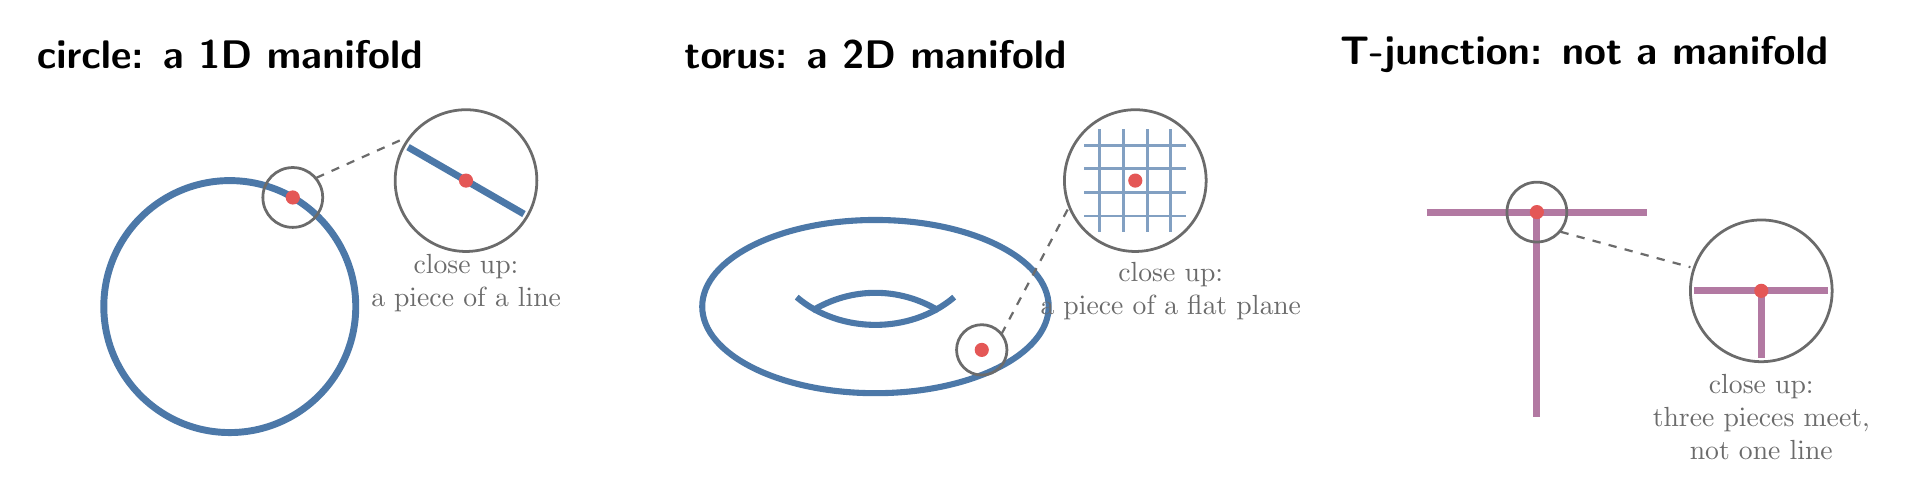
\begin{tikzpicture}[every node/.append style={font=\large}]
  % circle
  \node[title] at (0,3.2) {circle: a 1D manifold};
  \draw[cblue, line width=2.5pt] (0,0) circle (1.6);
  \fill[cred] (60:1.6) circle (0.09);
  \draw[cgrey, line width=1pt] (60:1.6) circle (0.38);
  \draw[cgrey, dashed, line width=0.8pt] ($(60:1.6)+(0.3,0.25)$) -- (2.25,2.15);
  \draw[cgrey, line width=1pt] (3.0,1.6) circle (0.9);
  \draw[cblue, line width=2.5pt] ($(3.0,1.6)+(150:0.85)$) -- ($(3.0,1.6)+(-30:0.85)$);
  \fill[cred] (3.0,1.6) circle (0.09);
  \node[cgrey, font=\normalsize, align=center] at (3.0,0.3) {close up:\\ a piece of a line};
  % torus
  \begin{scope}[xshift=8.2cm]
  \node[title] at (0,3.2) {torus: a 2D manifold};
  \draw[cblue, line width=2.2pt] (0,0) ellipse (2.2 and 1.1);
  \draw[cblue, line width=2.2pt] (-1.0,0.12) .. controls (-0.45,-0.35) and (0.45,-0.35) .. (1.0,0.12);
  \draw[cblue, line width=2.2pt] (-0.8,-0.05) .. controls (-0.3,0.25) and (0.3,0.25) .. (0.8,-0.05);
  \fill[cred] (1.35,-0.55) circle (0.09);
  \draw[cgrey, line width=1pt] (1.35,-0.55) circle (0.32);
  \draw[cgrey, dashed, line width=0.8pt] (1.6,-0.35) -- (2.45,1.25);
  \draw[cgrey, line width=1pt] (3.3,1.6) circle (0.9);
  \foreach \d in {-0.45,-0.15,0.15,0.45} {
    \draw[cblue!70, line width=1pt] (3.3+\d,0.95) -- (3.3+\d,2.25);
    \draw[cblue!70, line width=1pt] (2.65,1.6+\d) -- (3.95,1.6+\d);
  }
  \fill[cred] (3.3,1.6) circle (0.09);
  \node[cgrey, font=\normalsize, align=center] at (3.75,0.2) {close up:\\ a piece of a flat plane};
  \end{scope}
  % T junction
  \begin{scope}[xshift=16.6cm]
  \node[title] at (0.6,3.2) {T-junction: not a manifold};
  \draw[cpurple, line width=2.5pt] (-1.4,1.2) -- (1.4,1.2);
  \draw[cpurple, line width=2.5pt] (0,1.2) -- (0,-1.4);
  \fill[cred] (0,1.2) circle (0.09);
  \draw[cgrey, line width=1pt] (0,1.2) circle (0.38);
  \draw[cgrey, dashed, line width=0.8pt] (0.3,0.95) -- (1.95,0.5);
  \draw[cgrey, line width=1pt] (2.85,0.2) circle (0.9);
  \draw[cpurple, line width=2.5pt] (2.0,0.2) -- (3.7,0.2);
  \draw[cpurple, line width=2.5pt] (2.85,0.2) -- (2.85,-0.65);
  \fill[cred] (2.85,0.2) circle (0.09);
  \node[cgrey, font=\normalsize, align=center] at (2.85,-1.4) {close up:\\ three pieces meet,\\ not one line};
  \end{scope}
\end{tikzpicture}
\end{document}
